\documentclass[12pt]{article}

\usepackage{amsmath}

\usepackage{bookmark}

\usepackage{listings}
\usepackage[usenames,dvipsnames]{xcolor}

\usepackage{graphicx}

\usepackage{tikz}

\usepackage{amssymb}

\usepackage{makecell}

\usepackage{empheq}

\usetikzlibrary{quantikz}

\usepackage[rightcaption]{sidecap}

\usepackage{pgfplots}

\usepgfplotslibrary{statistics}

\pgfplotsset{compat=1.16}

\usepackage{hyperref}

\usepackage{verbatim}

\lstdefinelanguage{Julia}%
  {morekeywords={abstract,break,case,catch,const,continue,do,else,elseif,%
      end,export,false,for,function,immutable,import,importall,if,in,%
      macro,module,otherwise,quote,return,switch,true,try,type,typealias,%
      using,while},%
   sensitive=true,%
   alsoother={\$},%
   morecomment=[l]\#,%
   morecomment=[n]{\#=}{=\#},%
   morestring=[s]{"}{"},%
   morestring=[m]{'}{'},%
}[keywords,comments,strings]%

\lstset{%
    language         = Julia,
    basicstyle       = \fontsize{8}{13}\selectfont\ttfamily,
    keywordstyle     = \bfseries\color{blue},
    stringstyle      = \color{magenta},
    commentstyle     = \color{gray},
    showstringspaces = false,
}

\title{Computational Methods: Project 2}

\author{Ace Chun}

\begin{document}

\maketitle

\section{Function}
    \[-5.2z^2 + 176z + 1218 = 0\]
    The integral of this function between two points $a$ and $b$ will simply be the evaluation of 
    \[\left[-\frac{5.2}{3}z^3 + 88z^2 + 1218z\right]^{z = b}_{z = a}\]
    For the sake of code simplicity and to avoid needing the user to know the indefinite integral of the function 
    prior to calculation, an method from the MTH229 package was used to compute the ``true'' integral. Note that this would make 
    the error calculations relative approximate error, rather than relative true error; however, both formulas behave the same.

    For all methods, for the sake of testing, we wil choose the interval 
    \[[-10, 30]\]
    to estimate. This interval yields a true value of 70586.67 units squared.

\section{LRAM}
    The Left Rectangle Approximation Method (LRAM) approximates the area under a curve by taking the area of a rectangle for $n$ intervals. The height 
    of these rectangles is the function evaluated at the leftmost point in the given interval. This method was implemented in the following function:
    \begin{lstlisting}[language=julia]
function LRAM(func, left, right, n) 
    # using MTH229 and sympy to find the true value of the integral
    @syms x 
    true_val = integrate(func(x), (x, left, right))

    accumulator = 0 

    plot(func, left, right, framestyle=:zerolines)
    rectangle(w, h, l_x, l_y) = Shape(l_x .+ [0, w, w, 0], l_y .+ [0, 0, h, h])

    delta = (right - left) / n
    for i in 0:(n - 1)
        h = func(left + i * delta)
        accumulator += delta * h
        plot!(rectangle(delta, h, left + delta * i, 0), opacity=0.4, primary=false)
    end
    RRAM(p, -10, 30, 7, int_p)
    # relative true error calculation
    error = abs((true_val - accumulator) / true_val)

    println("Approximation: " * string(accumulator))
    println("True value: " * string(true_val))
    println("Error: " * string(error * 100) * "\%")
    savefig("images/LRAM.png")
end
    \end{lstlisting}
    For $ n= 7$, the approximation was visualized as 
    \begin{center}
        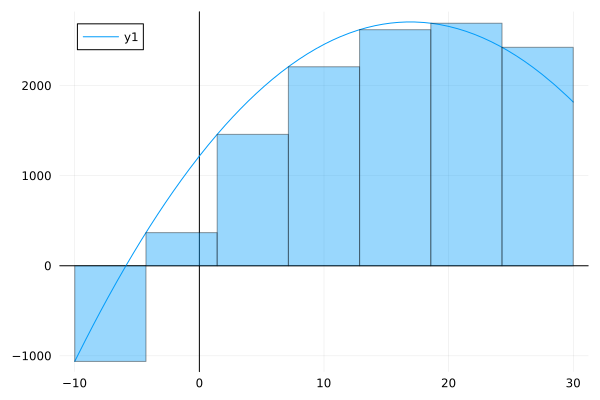
\includegraphics[scale=0.45]{images/LRAM_1.png}
    \end{center}
    This approximation yielded an absolute relative error of 13.26\%, where the estimated area under the curve 
    was computed to be 61226.12 units squared, compared to the ``true'' value of 70586.67 units squared. 

    Increasing the number of boxes that we have, or $n$, will make our estimate ``finer'' and thus generate a more accurate figure. 
    Using double the number of boxes ($n = 14$) yields
    \begin{center}
        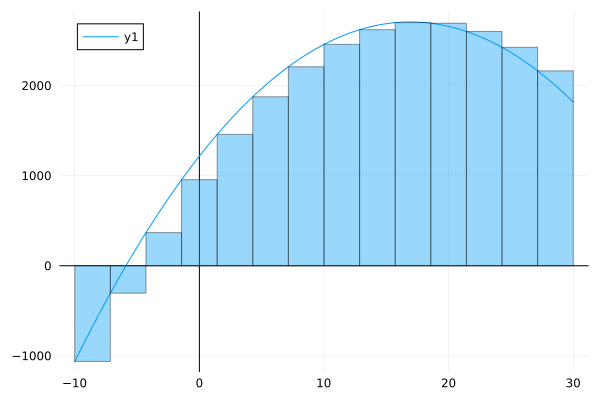
\includegraphics[scale=0.45]{images/LRAM_2.png}
    \end{center}
    This approximation has an error of only 6.22\% with an approximated value of 77683.27 units squared. As we can see, the amount of ``overhang'' and ``underhang'' from the boxes 
    significantly decreases with a greater number of boxes.

\section{RRAM}
    The Right Rectangle Approximation Method (RRAM) approximates the area under a curve by a 
    similar approach as the LRAM method. However, in RRAM, the height of the rectangle is instead the function evaluated at the 
    rightmost point in any given interval. 
    \begin{lstlisting}[language=julia]
function RRAM(func, left, right, n) 
    # using MTH229 and sympy to find the true value of the integral
    @syms x 
    true_val = integrate(func(x), (x, left, right))

    accumulator = 0
    plot(func, left, right, framestyle=:zerolines)
    rectangle(w, h, l_x, l_y) = Shape(l_x .+ [0, w, w, 0], l_y .+ [0, 0, h, h])

    delta = (right - left) / n
    for i in 0:(n-1)
        h = func(left + (i+1) * delta)
        accumulator += delta * h
        plot!(rectangle(delta, h, left + delta * i, 0), opacity=0.4, primary=false)
    end

    # relative true error calculation
    error = abs((true_val - accumulator) / true_val)

    println("Approximation: " * string(accumulator))
    println("True value: " * string(true_val))
    println("Error: " * string(error * 100) * "\%")
    
    savefig("images/RRAM.png")
end
    \end{lstlisting}
    Once again, using $n=7$ boxes yields an approximation like so:
    \begin{center}
        \includegraphics*[scale=0.45]{images/RRAM_1.png}
    \end{center}
    This approximation yielded a value of 77683.26 units squared, which has an error of around 10.05\%. 
    If we use $n=14$ boxes instead, 
    \begin{center}
        \includegraphics*[scale=0.45]{images/RRAM_2.png}
    \end{center}
    This yields a value of 74417.96 units squared, which has a relative error of 5.43\%.

\section{MRAM}
    The Midpoint Rectangle Approximation Method (MRAM) approximates the area under a curve with a similar approximation as the previous two, but uses the function evaluated 
    at the middle of the interval as the height for the box. 
    \begin{lstlisting}[language=julia]
function MRAM(func, left, right, n)
    @syms x # using MTH229 and sympy to find the true value of the integral
    true_val = integrate(func(x), (x, left, right))

    accumulator = 0

    function midpoint(l, r)
        return (l + r) / 2
    end
    
    plot(func, left, right, framestyle=:zerolines)
    rectangle(w, h, l_x, l_y) = Shape(l_x .+ [0, w, w, 0], l_y .+ [0, 0, h, h])
    delta = (right - left) / n

    for i in 0:(n-1)
        h = func(midpoint(left + i * delta, left + (i + 1) * delta))
        accumulator += delta * h
        plot!(rectangle(delta, h, left + delta * i, 0), opacity=0.4, primary=false)
    end

    # relative true error calculation
    error = abs((true_val - accumulator) / true_val)

    println("Approximation: " * string(accumulator))
    println("True value: " * string(true_val))
    println("Error: " * string(error * 100) * "\%")

    savefig("images/MRAM.png")
end
    \end{lstlisting}
    Using $n=7$ boxes yields
    \begin{center}
        \includegraphics*[scale=0.45]{images/MRAM_1.png}
    \end{center}
    This approximation is already remarkably close to the true value, with an approximation of 71152.65 units squared and an error of 
    0.80\%. Increasing the number of boxes to $n=14$ yields 
    \begin{center}
        \includegraphics*[scale=0.45]{images/MRAM_2.png}
    \end{center}
    This approximation yields an area of 70728.16 units squared, with an error percentage of 0.20\%.

\section{Lower bound}
    The lower bound approximation approximates the error by instead using the point where the function is lowest in the interval as the height of the rectangle. 
    To calculate this lower height, I reasoned that this lowest value must occur at either endpoint (where the derivative DNE) or a critical point (where derivative is equal to 0), should one exist in the interval.
    This is effectively an implementation of the Not the First Derivative Test (Blairism). To implement this, I took the height of a rectangle in any given interval 
    to be the minimum between the function evaluated at one of the endpoints or a critical point that exists inside of the interval.
    \begin{lstlisting}[language=julia]
function lower_approx(func, left, right, n)
    @syms x # using MTH229 and sympy to find the true value of the integral
    true_val = integrate(func(x), (x, left, right))
    critical_point = find_zero(func', left)

    delta = (right - left) / n
    plot(func, left, right, framestyle=:zerolines)
    rectangle(w, h, l_x, l_y) = Shape(l_x .+ [0, w, w, 0], l_y .+ [0, 0, h, h])

    accumulator = 0
    for i in 0:(n-1)
        # finding the lowest value, based on critical points
        if left + i * delta < critical_point && critical_point < left + (i+1) * delta
            h = min(func(critical_point), func(left + i * delta), func(left + (i+1) * delta))
        else 
            h = min(func(left + i * delta), func(left + (i + 1) * delta))
        end
        accumulator += delta * h
        plot!(rectangle(delta, h, left + delta * i, 0), opacity=0.4, primary=false)
    end

    # relative true error calculation
    error = abs((true_val - accumulator) / true_val)

    println("Approximation: " * string(accumulator))
    println("True value: " * string(true_val))
    println("Error: " * string(error * 100) * "\%")

    savefig("images/LowerRAM.png")

end
    \end{lstlisting}
    This method, using $n=8$ boxes, yields 
    \begin{center}
        \includegraphics*[scale=0.45]{images/LowerRAM_1.png}
    \end{center}
    This approximation results in an area of 58170.00 units squared, and an error percentage of around 17.59\%. 
    If we double the number of rectnagles, we see 
    \begin{center}
        \includegraphics*[scale=0.45]{images/LowerRAM_2.png}
    \end{center}
    which results in an approximation of 64551.25 units squared and an error percentage of 8.55\%.

\section{Summary}
    In summary, we see that in general, increasing the number of rectangles used in the approximation makes it more accurate to the true value of the area under the curve. 
    If we were given a function that did not have a closed-form integral, we would instead calculate error using the Relative Approximate Error formula, instead of the true relative error.

\end{document}